\documentclass{beamer}
\usepackage{amsmath,amssymb,amsthm,slashed, euscript}



\textwidth=110mm


\title{Hausdorff blowing-up of spectra of $C^*$-algebras and its applications}
\institute
{
Algebras in analysis
}

\author{Petr R. Ivankov  }



\theoremstyle{plain}
\newtheorem{defn}{Definition}
\newtheorem{rem}{Remark}
\newtheorem{exm}{Example}
\newtheorem*{claim}{Claim}
\newtheorem{prop}{Proposition}
\newtheorem{empt}[prop]{}%[section]
\newtheorem{lem}{Lemma}%[section]
\newtheorem{thm}{Theorem}%[section]



\newcommand{\A}{\mathcal{A}}
\newcommand{\be}{\begin{equation}}
\newcommand{\ee}{\end{equation}}
\newcommand{\Ga}{\Gamma}
\newcommand{\B}{\mathcal{B}}
\newcommand{\Cc}{\mathcal{C}}
\newcommand{\C}{\mathbb{C}}
\newcommand{\D}{\mathcal{D}}
\newcommand{\G}{\mathcal{G}}
\newcommand{\Hc}{\mathcal{H}}
\newcommand{\Lc}{\mathcal{L}}
\newcommand{\Pc}{\mathcal{P}}
\newcommand{\Sc}{\mathcal{S}}
\newcommand{\U}{\mathcal{U}}
\newcommand{\rar}{\rightarrow}
\newcommand{\Ef}{\mathbb{E}}
\newcommand{\desc}{\mathfrak{desc}}


%Uppercase Gothic characters
\newcommand{\gtA}{\mathfrak{A}}
\newcommand{\gtB}{\mathfrak{B}}
\newcommand{\gtM}{\mathfrak{M}}
\newcommand{\gtN}{\mathfrak{N}}
\newcommand{\gtP}{\mathfrak{P}}
\newcommand{\gtS}{\mathfrak{S}}

%Lowercase Gothic characters
\newcommand{\gtf}{\mathfrak{f}}
\newcommand{\gtg}{\mathfrak{g}}

%Bold Characters
\newcommand{\Cb}{\mathbb{C}}
\newcommand{\Nb}{\mathbb{N}}
\newcommand{\Rb}{\mathbb{R}}
\newcommand{\Zb}{\mathbb{Z}}

%Uppercase Greek characters
\newcommand{\Gm}{\Gamma}
\newcommand{\Te}{\Theta}
\newcommand{\Om}{\Omega}
\newcommand{\s}{ }

%Lowercase Greek characters
\newcommand{\al}{\alpha}
\newcommand{\gm}{\gamma}
\newcommand{\dl}{\delta}
\newcommand{\sg}{\sigma}
\newcommand{\ph}{\varphi}
\newcommand{\te}{\theta}
\newcommand{\ze}{\zeta}
\newcommand{\lift}{\mathfrak{lift}}
\newcommand{\eps}{\varepsilon}                    %% tensor product


\newcommand{\Id}{\mathrm{Id}}
\newcommand{\Aut}{\mathrm{Aut}}
\newcommand{\Coo}{{\mathrm{C}}^\infty}
\newcommand{\alg}{\mathrm{alg}}
\newcommand{\diag}{\mathrm{diag}}
\newcommand{\spinc}{\textbf{$spin^c$}}
\newcommand{\Hom}{\mathrm{Hom}}
\newcommand{\supp}{\mathrm{supp}}
\newcommand{\Ccl}{\mathbf{C}l}
\newcommand{\xto}{\xrightarrow}

\newcommand{\lto}{\longrightarrow}
\newcommand{\ox}{\otimes}
\newcommand{\nb}{\nabla}
\newcommand{\sS}{\mathcal{S}}
\newcommand{\Dn}{D\!\!\!\!/}
%\newcommand{\ij}{{i,j}}
\newcommand{\aC}{\ensuremath{\underline{\Cb}} }
\newcommand{\scp}[2]{\left\langle{#1},{#2}\right\rangle}
\newcommand{\op}[1]{J{#1}J^\dag}
\newcommand{\sA}{\mathcal{A}} 
\newcommand{\sB}{\mathcal{B}}       %%
\newcommand{\sC}{\mathcal{C}}       %%
\newcommand{\sD}{\mathcal{D}}       %%
\newcommand{\sE}{\mathcal{E}}       %%
\newcommand{\sF}{\mathcal{F}}       %%
\newcommand{\sG}{\mathcal{G}}       %%
\newcommand{\sH}{\mathcal{H}}       %%
\newcommand{\sI}{\mathcal{I}}       %%
\newcommand{\sJ}{\mathcal{J}}       %%
\newcommand{\sK}{\mathcal{K}}       %%
\newcommand{\sL}{\mathcal{L}}       %%
\newcommand{\sM}{\mathcal{M}}       %%
\newcommand{\sN}{\mathcal{N}}       %%
\newcommand{\sO}{\mathcal{O}}       %%
\newcommand{\sP}{\mathcal{P}}       %%
\newcommand{\sQ}{\mathcal{Q}}       %%
\newcommand{\sR}{\mathcal{R}}       %%
\newcommand{\sT}{\mathcal{T}}       %%
\newcommand{\sU}{\mathcal{U}}       %%
\newcommand{\sV}{\mathcal{V}}       %%
\newcommand{\sX}{\mathcal{X}}       %%
\newcommand{\sY}{\mathcal{Y}}       %%
\newcommand{\sZ}{\mathcal{Z}}       %%
\newcommand{\N}{\mathbb{N}}                  %% 

\renewcommand{\a}{\alpha}     
\newcommand{\la}{\lambda}     
\newcommand{\La}{\Lambda}
\newcommand{\bt}{\beta}           %% short for  \beta
 
 	\newcommand{\bean}{\begin{eqnarray*}}
 	\newcommand{\eean}{\end{eqnarray*}}
    
\newcommand{\bydef}{\stackrel{\mathrm{def}}{=}}  
\newcommand{\hookto}{\hookrightarrow}        %% abbreviation
  \usepackage{graphicx}
  \graphicspath{ {./images/} }
  \usepackage{tikz}
\usetikzlibrary{calc,trees,positioning,arrows,chains,shapes.geometric,%
	decorations.pathreplacing,decorations.pathmorphing,shapes,%
	matrix,shapes.symbols}
  
  \tikzset{
  	>=stealth',
  	punktchain/.style={
  		rectangle, 
  		rounded corners, 
  		% fill=black!10,
  		draw=black, very thick,
  		text width=10em, 
  		minimum height=3em, 
  		text centered, 
  		on chain},
  	line/.style={draw, thick, <-},
  	element/.style={
  		tape,
  		top color=white,
  		bottom color=blue!50!black!60!,
  		minimum width=8em,
  		draw=blue!40!black!90, very thick,
  		text width=10em, 
  		minimum height=3.5em, 
  		text centered, 
  		on chain},
  	every join/.style={->, thick,shorten >=1pt},
  	decoration={brace},
  	tuborg/.style={decorate},
  	tubnode/.style={midway, right=2pt},
  }
\begin{document}
%\titlepage
\begin{frame}
  \titlepage
\end{frame}
\begin{frame}
\begin{definition}\label{blowing_u_defn}\alert{Petr Ivankov.}
	If $A$ is a $C^*$-algebra then \alert{Hausdorff blowing-up} is an injective inclusion  $C_0\left( \sY\right) \subset M\left( A\right)$ such that:
\begin{enumerate}
	\item[(a)] $C_c\left( \sY\right)A$ is dense in $A$,
	\item [(b)]  $AC_c\left( \sY\right)$ is dense in $A$.
\end{enumerate} 
\end{definition}
\begin{rem}
Both conditions (a) and (b) are equivalent to each other and used for convenience.
\end{rem}
\begin{rem}
	If $C_0\left( \sY\right)$ is within a center of $M\left( A\right)$ then $\sY$ is the spectrum of $A$.
\end{rem}
\begin{rem}
	The "blowing-up" etymology comes from the algebraic geometry, where it means a map from nonsingular variety  onto a variety with singularities.
\end{rem}

\end{frame}
\section{Basic example}
\begin{frame}
	Basic example $$C_c\left(M \right) \subset M\left( C^*\left(M, \sF \right)\right) $$  where 
	$\left(M, \sF \right)$ is a foliated manifold and  $C^*\left(M, \sF \right)$ is a $C^*$-algebra of foliation. The spectrum of $C^*\left(M, \sF \right)$ is a set of leaves, and there is the natural map from $M$ to the spectrum.
\\
\includegraphics[scale=0.25]{Untitled.png}
\begin{rem}
There are different of versions of $ C^*\left(M, \sF \right)$, all of them are being studied.
\end{rem}
\end{frame}
\begin{frame}
There are several  analogies  with spectrum.\\
Simplest analogy\\
Spectrum
$$
C_0\left(\sX_1\sqcup ...\sqcup \sX_n \right) \cong C_0\left(\sX_1 \right) \oplus ...\oplus C_0\left(\sX_n \right) 
$$
Blowing-up
\bean
C_0\left( \sY_1\sqcup ...\sqcup \sY_n\right)\subset M\left( A\right)\quad   
A \cong A_1\oplus ...\oplus A_n,\\
\forall j \in \{1,...,n\}\quad C_0\left(\sU_j \right) \subset M\left(A_j \right). 
\eean

\end{frame}

\begin{frame}
	\begin{thm}\label{pedersen_ideal_thm} \alert{Pedersen G.K.}
		% THEOREM 5.6.1
		For each $C^*$-algebra $A$ there is a dense hereditary ideal $K(A)$,
		which is minimal among dense ideals.
		
	\end{thm}
	\begin{proof}
		Let $K(]0, \infty [)$ denote the set of continuous functions on $]0, \infty [$ with 
		compact support and define 
		\be\label{pedersen_k0_eqn}
		K\left( A \right)_0 \bydef \left\{f\left(x\right) \left|x \in A_+, \quad f \in K(]0, \infty [) \right.\right\}.
		\ee
		Let 
		\be\label{pedersen_k_plus_eqn}
		K\left( A \right)_+ \bydef \left\{x \in A_+ \left|x \le \sum_{j = 1}^nx_j, \quad x_j \in  	K\left( A \right)_0\right.\right\}, 	
		\ee
		so that $	K\left( A \right)_+$ is the smallest hereditary cone  containing $K\left( A \right)_0$. If $K(A)$ 
		is  the algebraic  $\C$-linear span of $K(A)_+$ then $K(A)$,
		which is minimal among dense ideals. The full  proof is  described in Pedersen's book.
	\end{proof}
	
\end{frame}

\begin{frame}
	The above ideal is said to be \alert{Pedersen's ideal}. It is  proven by \alert{Ivankov P.R.} that $f \in K(]0, \infty [)$ can be replaced with the continuous functions given by
		$$
		f_\eps\left( x\right)  \bydef\left\{
		\begin{array}{c l}
			0 &x \le \eps \\
			x - \eps & x > \eps
		\end{array}\right.
	$$
	where $\eps > 0$.
\end{frame}


\begin{frame}
	If $A$ is a $C^*$-algebra with Hausdorff spectrum then for any $a\in A$ there is generated by $a$ closed two sided ideal $I\subset A$. The ideal yields an open subset of the spectrum of $A$ the closure of this set is the \alert{support} $\supp~a$ of $a$. It is well known  that if $a \in K\left(A \right)$ then  $\supp~a$ is compact. There is a generalization of this result.
\end{frame}
\begin{frame}
\begin{definition}\label{blowing_ideals_au_ua_defn}
	Let  $ C_0\left(\sY\right)\subset  M\left( A\right) $ be  Hausdorff blowing-up of $A$, and let $\sU \subset \sY$ be an open subset. Both   left and right  closed ideals $A_\sU$  and $_\sU A$ of $A$ (cf. Definition  generated by sets 	$AC_0\left( \sU\right)$ and $C_0\left( \sU\right)A$ are the \alert{left} $\sU$-\alert{ideal} and the \alert{right} $\sU$-\alert{ideal} respectively. A hereditary $C^*$-subalgebra of $A$
	\be\label{blowing_hereditary_u_eqn} 
	\begin{split}
		_\sU A_\sU \bydef		_\sU A\cap  A_\sU = A^*	_\sU \cap  A_\sU
	\end{split}
	\ee	
	is the \alert{hereditary} $\sU$-\alert{subalgebra}.
	
	\end{definition}
	
	\begin{definition}\label{blowing_support_defn}
		If $C_0\left( \sY\right) \subset M\left(A \right)$ is    {Hausdorff blowing-up} of $A$,  $a \in A$ and
		$
		\sU_a \bydef\bigcap 
		\left\{\left.{\sU} \subset \sX\right| a\in~_\sU A_{\sU} \right\}
		$
		then the  closure $\sV_a$  of $\sU_a$ is said to be the \alert{support} of $a$. We write $\supp~ a \bydef \sV_a$. This definition is a generalization of the definition of support in case of $C^*$-algebra with Hausdorff spectrum. 
	\end{definition}
	
\end{frame}

\begin{frame}
	\begin{lemma}\label{blowing_pedersen_compact_lem}
		If  $C_0\left( \sY\right)\hookto M\left( A\right)$ is Hausdorff blowing-up and $a\in A$ belongs to the Pedersen's ideal $K\left(A \right)$  then the support of $a$  is compact.
	\end{lemma}
\begin{proof}	
If $a \in K\left(A\right)_0$  then  there is $\eps > 0$ and $b \in A_+$ such that $a = f_\eps \left( b\right)$. On the other hand  there is a positive element  $c= fbf\in  A_+$  such that  $f\in C_c\left(\sY \right)$, $\left\|f \right\|=1 $, $c < b$, $\left\|c - b \right\|  < \eps/2$, and $\supp~ c\subset \supp ~f$ is compact.
If $a \le c$ does not hold and $\rho: A \hookto B\left(H \right)$ is a faithful  nondegenerate representation  then there is $\xi \in H$ such that
\bean\label{blowing_ac_eqn}
\forall \xi \in H \quad \left( \xi, \rho\left( a \right) \xi\right) > \left( \xi, \rho\left( c \right) \xi\right)
\eean
From $\left\|c - b \right\|  < \eps/2$ if follows that
\bean
\forall \xi \in H  \quad \left\| \xi \right\| = 1\quad \Rightarrow\quad  \left|\left( \xi, \rho\left( b \right) \xi\right)-\left( \xi, \rho\left( c \right) \xi\right) \right| < \eps/2
\eean
\end{proof}

\end{frame}
\begin{frame}
On the other hand from $a =f_\eps \left( b\right)> 0$ it follows that there is $\xi \in H$ and $\la \in \mathbf{R}_+$ such that
\bean
\left\| \xi \right\| = 1,\\
\rho\left(a \right) \xi = \la \xi,\\
\rho\left(b \right)\xi = \left( \la+\eps \right) \xi,\\
\rho\left(a \right)\xi = \la  \xi,\\
\left( \xi, \rho\left( b \right) \xi\right) - \left( \xi, \rho\left( a \right) \xi\right)= \\=\eps
\left( \xi, \rho\left( c \right) \xi\right)- \left( \xi, \rho\left( a \right) \xi\right)> \frac{\eps}{2}
\eean

Above condition contradicts with
$$
\left|\left( \xi, \rho\left( b \right) \xi\right)-\left( \xi, \rho\left( c \right) \xi\right) \right| < \eps/2
$$
so $a \le c$.
If $\supp a \subsetneqq \supp c$ then there is a nonempty  open set  $\sU \subset \supp a\setminus \supp c$. For any $f \in C_0\left(\sU \right)\setminus \{0\}$ one has
\bean
faf^* > 0,\\
fcf^* = 0.
\eean
\end{frame}
\begin{frame}
However it is impossible since $a \le c$, so $\supp~ a \subsetneqq \supp ~c$ is not true and $\supp a \subset\supp c$. Thus the set $\supp a$ is a closed subset of the compact set $\supp~ c$ therefore $\supp~ a$ is compact. Using this fact and the definition of the Pedersen's ideal we conclude that $\supp~ a$ is compact for any $a \in K\left( A\right)$. 
	
	
\end{frame}

\begin{frame}
Coverings of $C^*$-algebras
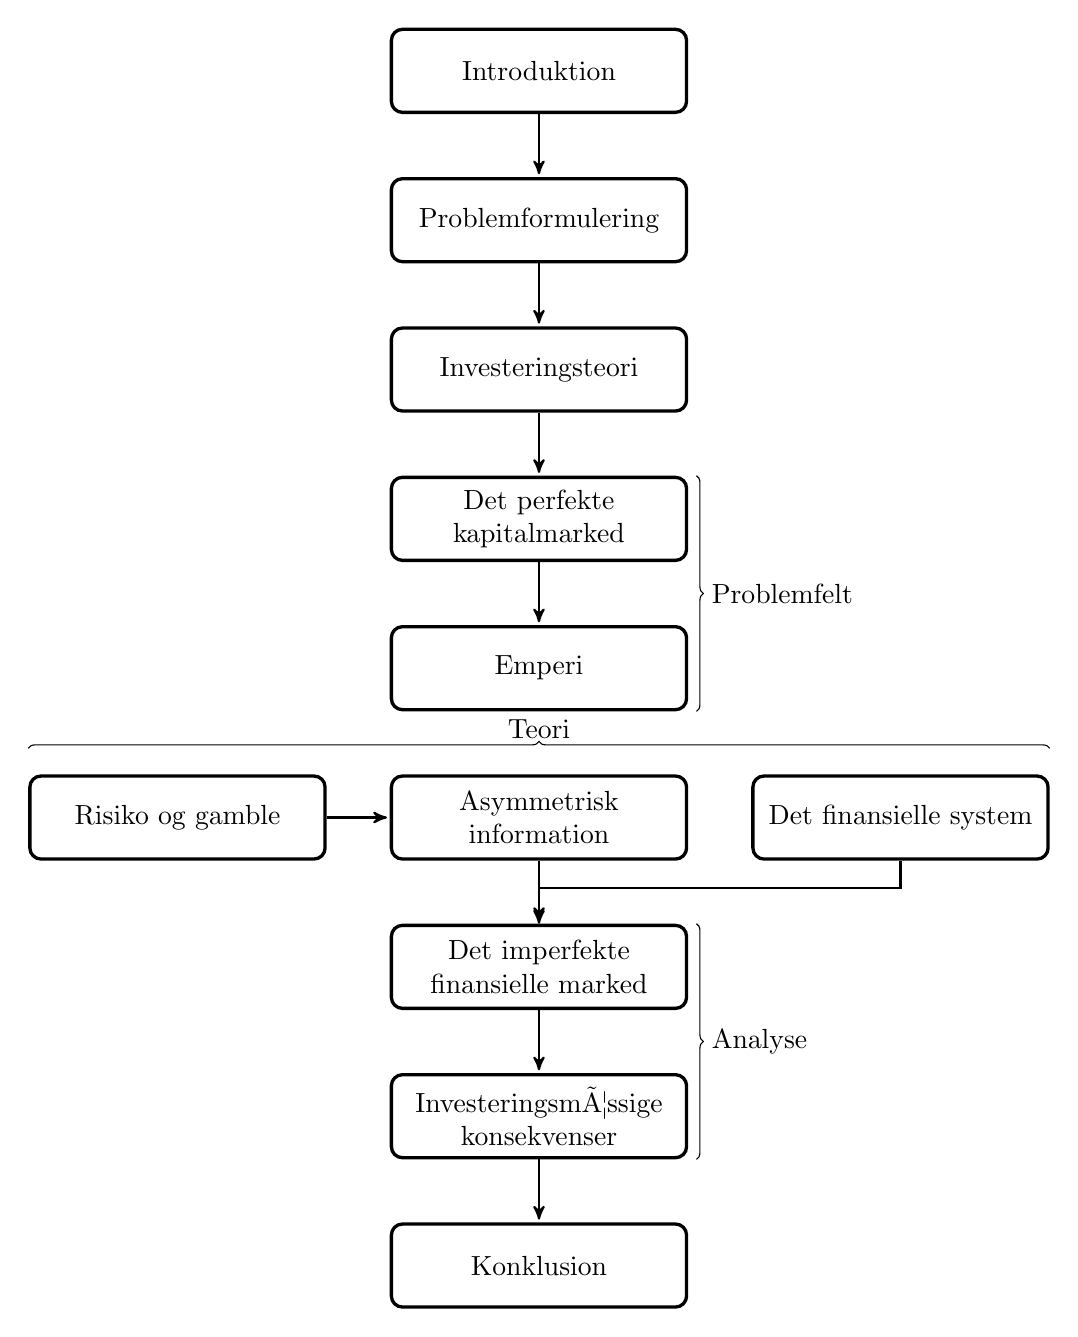
\begin{tikzpicture}
	[node distance=.8cm,
	start chain=going below,]
	\node[punktchain, join] (intro) {Introduktion};
	\node[punktchain, join] (probf)      {Problemformulering};
	\node[punktchain, join] (investeringer)      {Investeringsteori};
	\node[punktchain, join] (perfekt) {Det perfekte kapitalmarked};
	\node[punktchain, join, ] (emperi) {Emperi};
	\node (asym) [punktchain ]  {Asymmetrisk information};
	\begin{scope}[start branch=venstre,
		%We need to redefine the join-style to have the -> turn out right
		every join/.style={->, thick, shorten <=1pt}, ]
		\node[punktchain, on chain=going left, join=by {<-}]
		(risiko) {Risiko og gamble};
	\end{scope}
	\begin{scope}[start branch=hoejre,]
		\node (finans) [punktchain, on chain=going right] {Det finansielle system};
	\end{scope}
	\node[punktchain, join,] (disk) {Det imperfekte finansielle marked};
	\node[punktchain, join,] (makro) {Investeringsmæssige konsekvenser};
	\node[punktchain, join] (konk) {Konklusion};
	% Now that we have finished the main figure let us add some "after-drawings"
	%% First, let us connect (finans) with (disk). We want it to have
	%% square corners.
	\draw[|-,-|,->, thick,] (finans.south) |-+(0,-1em)-| (disk.north);
	% Now, let us add some braches. 
	%% No. 1
	\draw[tuborg] let
	\p1=(risiko.west), \p2=(finans.east) in
	($(\x1,\y1+2.5em)$) -- ($(\x2,\y2+2.5em)$) node[above, midway]  {Teori};
	%% No. 2
	\draw[tuborg, decoration={brace}] let \p1=(disk.north), \p2=(makro.south) in
	($(2, \y1)$) -- ($(2, \y2)$) node[tubnode] {Analyse};
	%% No. 3
	\draw[tuborg, decoration={brace}] let \p1=(perfekt.north), \p2=(emperi.south) in
	($(2, \y1)$) -- ($(2, \y2)$) node[tubnode] {Problemfelt};
\end{tikzpicture}
\end{frame}

\end{document}























